\chapter{Implementación}
\label{Implementación}

\section{Introducción}
En este capítulo se describen los procedimientos de implementación que se realizaron, expuestos de forma cronológica, es decir a medida que se avanzaba con el proyecto, comenzando con la configuración del ambiente de trabajo, después el armado del dataset a partir de las imágenes/datos obtenidos, para luego entrenar el modelo con la correcta monitorización de los resultados y por último, desplegar el software final.

\begin{figure}
    \centering
    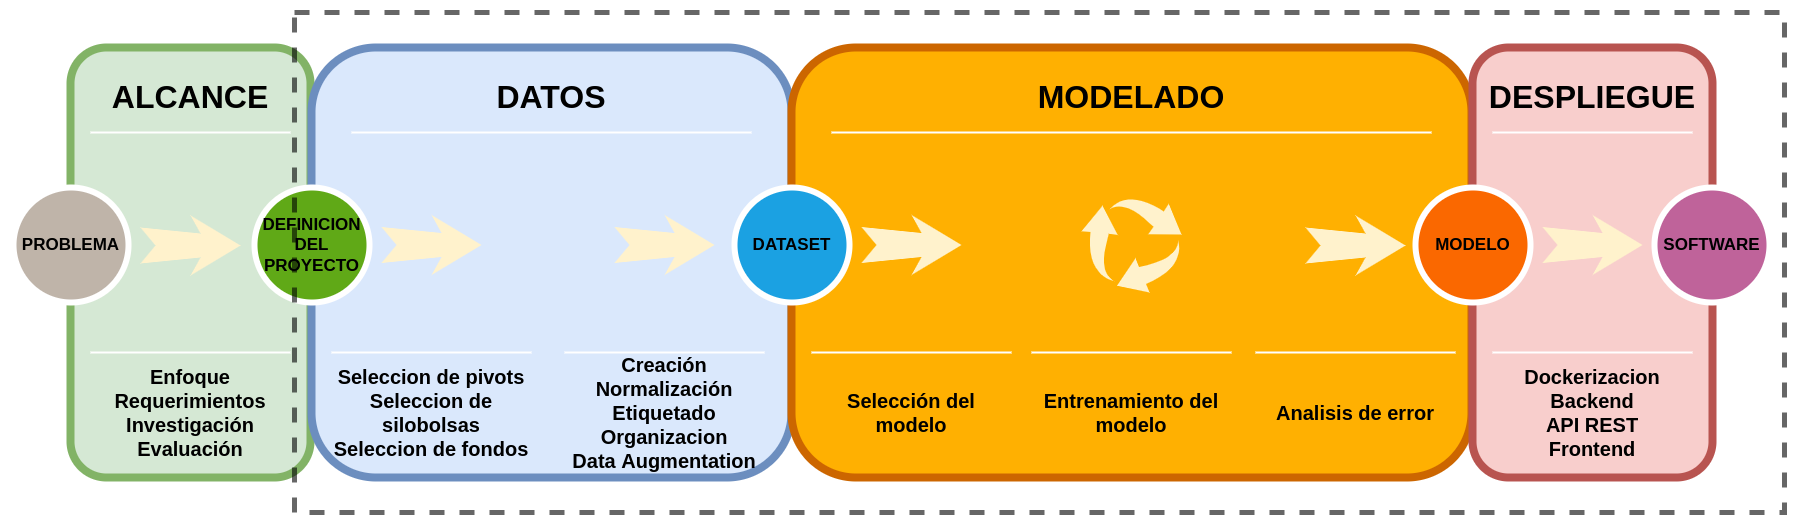
\includegraphics[width=1.2\textwidth,center]{img/Wokflow - datos_modelado_despliegue.drawio.png}
    \caption{Workflow: Implementación}
    \label{fig:workflow - implementacion}
\end{figure}

\subsection{Entornos de trabajo}
Para el desarrollo de este proyecto, se utilizaron dos computadoras con el sistema operativo Linux instalado (distintas distribuciones de Ubuntu), con conexión a internet y además de la súper computadora de la UNC (Universidad Nacional de Córdoba) Nabucodonosor (\textit{Nabu}) \cite{nabucodonosor} para el entrenamiento. A continuación se detalla el hardware que conforma el clúster:
\begin{itemize}
    \item \textbf{CPU}: Xeon E5-2680v2 (x2)
    \item \textbf{RAM}: 64 GB
    \item \textbf{GPU}: NVIDIA GTX 1080Ti (3x)
    \item \textbf{Almacenamiento}: 3 TiB + 240 GiB
\end{itemize}

El proyecto se realizó en gran parte de forma remota, usando las computadoras personales para conectarse a \textit{Nabu} usando un túnel SSH \cite{ssh}, lo que brindaba la posibilidad de disponer de un gran poder de computo sin largas colas de espera ni limitaciones de tiempo, desde cualquier lugar. Sin embargo, surgieron algunas limitaciones, sobre todo relacionadas a la ausencia de una  interfaz gráfica al trabajar desde una consola; por lo que para ciertas tareas fue necesario usar las PCs locales. A continuación se detallan las tareas del proyecto que se llevaron a cabo en cada entorno:\\

\textbf{Entorno PC}
\begin{itemize}
    \item Generación del dataset básico: Usando software para acceder a fuentes de imágenes satelitales \textit{QGIS}, \textit{Google Earth}, editor de imágenes \textit{Gimp} y etiquetador manual \textit{YOLO Annotation Tool}.
    \item Programación de código fuente: Se utilizo un editor de texto que modificara remotamente los archivos en \textit{Nabu}.
    \item Prueba del BackEnd: Se hizo uso de navegadores web y del software \textit{Postman} para probar el backend, haciendo uso del \textit{re-direccionamiento de puertos}.
    \item Diseño y prueba de FrontEnd: Se accedía a la página web (el frontend de este proyecto) haciendo uso del re-direccionamiento de puertos.\\
\end{itemize}

\textbf{Entorno Nabucodonosor}:
\textit{Las siguientes tareas se ejecutaban en \textit{Nabu} a través de una consola conectada por un túnel SSH.}
\begin{itemize}
    \item Generación del dataset aumentado: Usando un script en Python personalizado se extendió el dataset básico ``manual'' con el objetivo de mejorar la performance del modelo. 
    \item Entrenamiento del modelo: Se ejecutó el entrenamiento del modelo usando diferentes versiones de dataset e hiper-parámetros hasta lograr resultados satisfactorios.
    \item Ejecución de la Detección: Todas las detecciones se ejecutan en el clúster, ya sea para pruebas manuales como para ejecuciones disparadas por el Backend.
    \item Ejecución del BackEnd: Se dejó corriendo un contenedor Docker con el backend basado en Python usando el framework \textit{Flask} el cual recibía consultas con imágenes para ser analizadas por el modelo.
    \item Ejecución del FrontEnd: Se dejó corriendo otro contenedor Docker con el frontend basado en JavaScript usando el framework \textit{Bootstrap} y HTML. El mismo dejaba corriendo un servidor con el frontend para ser accedido por cualquiera (teóricamente) y éste realizaba las consultas al backend con el modelo en ejecución. \textit{Aclaración}: Debido a limitaciones por seguridad del clúster este frontend solo fue accedido desde las PCs usando \textit{re-direccionamiento de puertos}.
\end{itemize}

\subsubsection{Configuración Nabucodonosor}
Lo principal para comenzar a desarrollar y trabajar sobre un modelo de Machine Learning es disponer del firmware y software para hacer uso del poder de computo, en particular, de las tarjetas gráficas. Para eso, un enfoque práctico es hacer uso de un contenedor \textit{Docker} sobre el cual  instalar librerías y dependencias que permitan realizar el desarrollo sin alterar el estado \textit{por defecto} del clúster para que el resto de los usuarios del mismo no se vean afectados. De esta forma se trabajó de manera encapsulada dentro de diferentes contenedores Docker obtenidos en \textit{DockerHub} \cite{dockerhub}, configurados de tal manera que cumplieran diferentes propósitos particulares.\\

\paragraph{Machine Learning \& Backend Docker}
Posee la siguiente configuración:
\begin{itemize}
    \item Driver Nvidia: Para hacer uso de los núcleos \textit{CUDA} \cite{cuda} disponibles en las 3 tarjetas gráficas.
    \item Python 3: Se le sumaron a las librerías pre-instaladas en el contenedor las siguientes librerías y frameworks:
    \begin{itemize}
        \item Anaconda: Framework basado en Python orientado a Machine Learning.
        \item Librerías:
        \begin{table}[h!]
            \centering
            \begin{tabular}{ | m{5cm} | m{4cm} |}
                \hline
                \textbf{Descripción o Uso} & \textbf{Librerías} \\
                \hline
                 Para Machine Learning      &   \begin{itemize}
                                                    \item matplotlib
                                                    \item numpy
                                                    \item opencv
                                                    \item Pillow
                                                    \item PyYAML
                                                    \item requests
                                                    \item scipy
                                                    \item torch
                                                    \item torchvision
                                                    \item tqdm
                                                \end{itemize}\\
                \hline
                Para inicio de sesión o Logueo                 &   \begin{itemize}
                                                    \item tensorboard
                                                \end{itemize}\\
                \hline
                Para Gráficas               &   \begin{itemize}
                                                    \item seaborn
                                                    \item pandas
                                                \end{itemize}\\
                \hline
                Para Backend                &   \begin{itemize}
                                                    \item flask
                                                    \item pyunpack
                                                    \item flask\_cors
                                                \end{itemize}\\
                \hline
                Para Monitoreo de Recursos  &   \begin{itemize}
                                                    \item htop
                                                \end{itemize}\\
                \hline
            \end{tabular}\\
            \caption{Librerías Backend}
            \label{librerias-be}
        \end{table}
    \end{itemize}
\end{itemize}
Además, para usar el mismo contenedor para ejecutar diferentes tareas con librerías incompatibles, se hizo uso de entornos virtuales usando \textit{VirtualEnv} \cite{virtualenv}. Se configuraron los siguientes entornos virtuales:
\begin{itemize}
    \item \textit{yolo-v5}: Para correr el modelo (entrenamiento y detección).
    \item \textit{yolo-annotation-tool}: Para correr el script que levantaba la interfaz gráfica para etiquetar imágenes manualmente.
\end{itemize}

\paragraph{Frontend Docker}
El contenedor en donde se despliega la interfaz gráfica posee la siguiente configuración:
\begin{itemize}
    \item JavaScript
    \item CSS
    \item HTML
    \item Bootstrap
\end{itemize}

\subsection{Dataset}
En esta sección se detallan las tareas y mecanismos utilizados para generar el dataset con el que se entrenó el modelo.
\subsubsection{Data Augmentation}
Las redes neuronales convolucionales necesitan una enorme cantidad de imágenes para entrenar de forma efectiva el modelo. Esta técnica permite incrementar el rendimiento y robustez del modelo \cite{dataaug} y se realiza aplicando diferentes transformaciones a las imágenes como invertirlas, zoom, rotaciones entre otras dando una mayor generalización y una reducción del overfitting o sobreajuste.

\begin{figure}
    \centering
    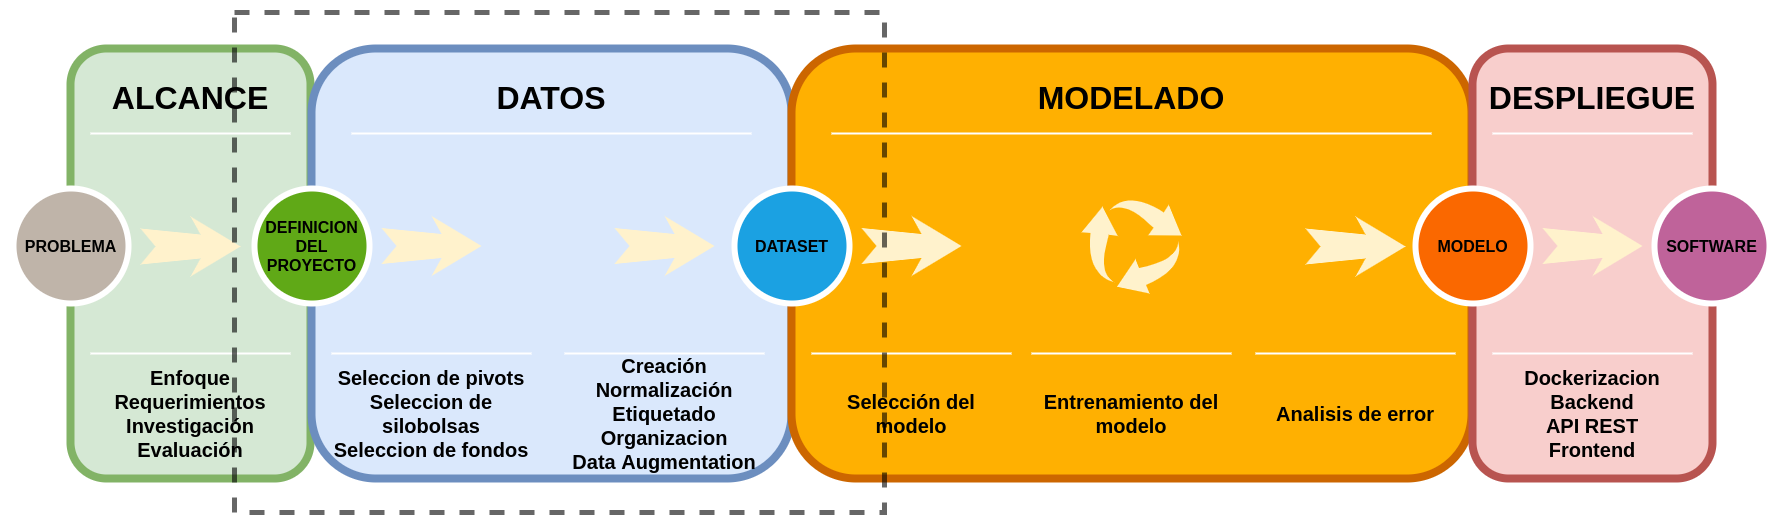
\includegraphics[width=1.2\textwidth,center]{img/Wokflow - datos.drawio.png}
    \caption{Workflow: Etapa de Datos}
    \label{fig:workflow - datos}
\end{figure}



Para el dataset se tomaron imágenes de silobolsas y pivotes de riego, y a mano se recortaron solo los objetos de las mismas, para así crear plantillas con fondo transparente en formato PNG (RGBA, donde A viene de \textit{Alpha} y se corresponde con el nivel de transparencia). Por otro lado se obtuvieron imágenes satelitales de diversos lugares del territorio argentino sin una determinada lógica, con el objetivo de conformar un conjunto de ``fondos'' sobre los cuales luego se combinarían con las plantillas de objetos. Para la generación de un dataset aumentado se programó un script en Python, el cual, toma todas las plantillas, las rota en un ángulo aleatorio y las posiciona en diversos lugares de un determinado fondo. De la combinación lineal de todos los fondos y todas las plantillas y sus alteraciones, surge un dataset lo suficientemente basto como para poder entrenar el modelo YOLO. Este script, además, se encarga de generar automáticamente los archivos de etiquetas para cada imagen nueva.

\subsubsection{Formatos}
Uno de los modelos con los que se trabajó en un principio, admitia el dataset de entrenamiento en formato \textit{TFRecord}. El mismo se generaba a partir correr un script en Python: \textit{YOLOToTFRecords} \cite{yolototfrecords}.
Este código fuente fue modificado para admitir archivos formato CSV y, a partir del mismo, generar el archivo TFRecord. Este es un formato especial creado por \textit{TensorFlow} para almacenar el dataset en formato binario.

Finalmente en el modelo final YOLOv5, solo bastaba con configurar el directorio donde se ubicaban las imágenes y sus etiquetas para poder entrenarlo.


\subsection{Entrenamiento}
\begin{figure}
    \centering
    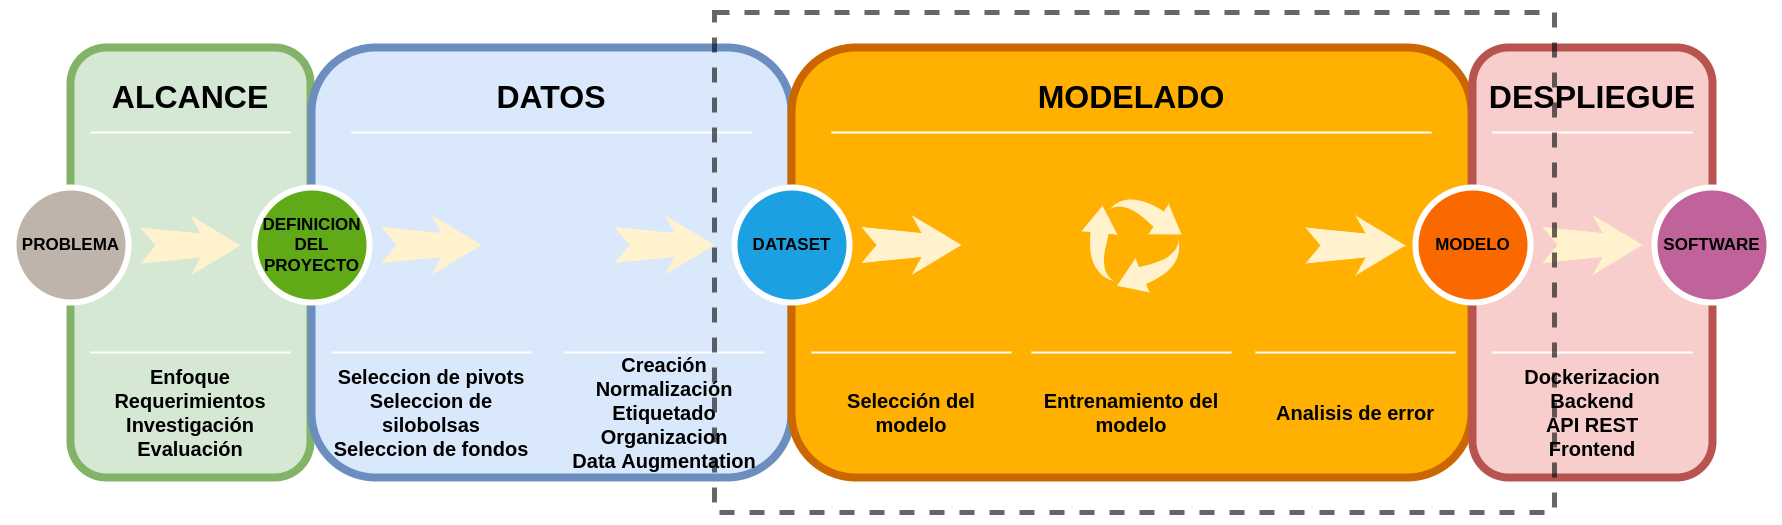
\includegraphics[width=1.2\textwidth,center]{img/Wokflow - modelado.drawio.png}
    \caption{Workflow: Etapa de Modelado}
    \label{fig:workflow - modelado}
\end{figure}
En esta etapa se procedió a entrenar el modelo utilizando el dataset generado. El proceso de entrenamiento consta de iterar una inmensa cantidad de veces sobre el dataset de entrenamiento, para que así, la red neuronal por la que esta compuesta el modelo, ``aprenda'' a detectar correctamente. Es un proceso repetitivo, en el cual, poseer un gran poder de computo reduce los tiempos de entrenamiento hasta llegar a un resultado aceptable. Para determinar cuándo un resultado es lo suficientemente bueno, es en donde se utilizan diferentes métricas para realizar pruebas.


\subsection{Pruebas}
En esta sección se expondrán y explicarán diferentes diagramas y gráficos, en base a las pruebas de validación y testeo que se realizaron sobre el modelo de Machine Learning. Cabe destacar que esta etapa conforma, junto con el entrenamiento, un proceso cíclico, el cual se repite hasta lograr los resultados esperados. \\
Se detalla a continuación algunos conceptos para comprender las métricas seleccionadas para valorar el funcionamiento del modelo, junto con sus correspondientes diagramas:

\subsubsection{Precisión}
Es la proporción de observaciones positivas predichas correctamente (verdadero positivo) sobre el total de predicciones realizadas. Su fórmula es:  \[Precisión=\frac{TP}{TP + FP}\]
\\
Donde:\\
TP: Truth Positive - Verdadero Positivo\\
FP: False Positive - Falso Positivo\\

Es decir, la precisión mide que tan preciso son las predicciones de nuestro modelo en base a un porcentaje de las predicciones correctas.\\

\textit{Ejemplo}:
La precisión representa el ratio entre verdaderos positivos y número total de positivos predichos. Por ejemplo, si el modelo detectó 5 pivotes de riego de los cuales 4 realmente lo eran, la precisión ha sido de 4 / 5 = 0.8.\\
El clasificador ideal tendría una precisión de 1, ya que todas las predicciones positivas serían verdaderas.
De forma equivalente, el peor clasificador posible, tendría una precisión de 0, ya que todas las predicciones positivas serían falsas.

\newpage
\textbf{Resultado obtenido}\\

En la Figura \ref{fig:precision}, podemos observar la curva de precisión obtenida para la detección de Silobolsas y Riegos por Pivot desde la Epoch (ciclo de entrenamiento) 1 al 100 y de la Epoch 101 a la 700. 
\begin{figure}[h!]
    \centering
    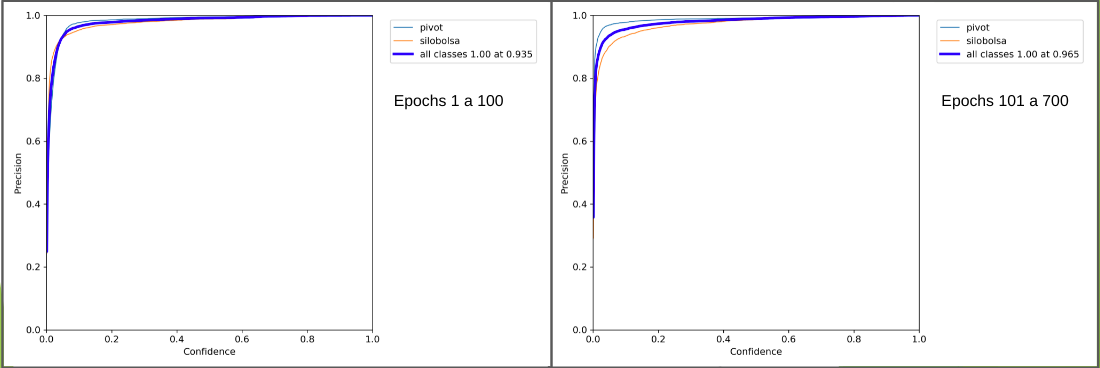
\includegraphics[width=1\textwidth]{img/Precision.png}
    \caption{Precisión}
    \label{fig:precision}
\end{figure}

\subsubsection{Recall o Sensibilidad} 
Es la proporción de observaciones positivas predichas correctamente con respecto a todas las observaciones en la clase real, es decir, mide la capacidad del modelo de detectar casos positivos, en este caso,
objetos que pertenezcan a alguna de las clases del dataset, ya sea Pivot o Silobolsa. Su fórmula es:  \[Recall=\frac{TP}{TP + FN}\]  

Por lo tanto \textbf{recall} es un porcentaje de los casos positivos correctamente acertados.\\

\textit{Ejemplo}:
La exhaustividad (recall en inglés, aunque también se conoce como sensibilidad o sensitivity, y TPR o True Positive Rate) de una clasificación es el ratio entre los verdaderos positivos (los que se han detectado) y los positivos reales (los hayamos detectado o no).\\
La exhaustividad sería el número de pivotes de riego detectados, dividido por el número de pivotes de riego reales totales: si hemos detectado 3 y había 5, la exhaustividad ha sido de 3 / 5 = 0.6. \\
El clasificador ideal tendría una exhaustividad de 1, pues todos los positivos reales serían detectados como positivos (verdaderos positivos).\\
El peor clasificador posible tendría una exhaustividad de 0, pues ninguno de los positivos reales sería identificado como positivo.

\newpage
\textbf{Resultado obtenido}\\
 
En la Figura \ref{fig:recall} podemos observar la curva de Recall obtenida para la detección de Silobolsas y Pivot desde la Epoch 1 al 100 y de la Epoch 101 a la 700.

\begin{figure}[h!]
    \centering
    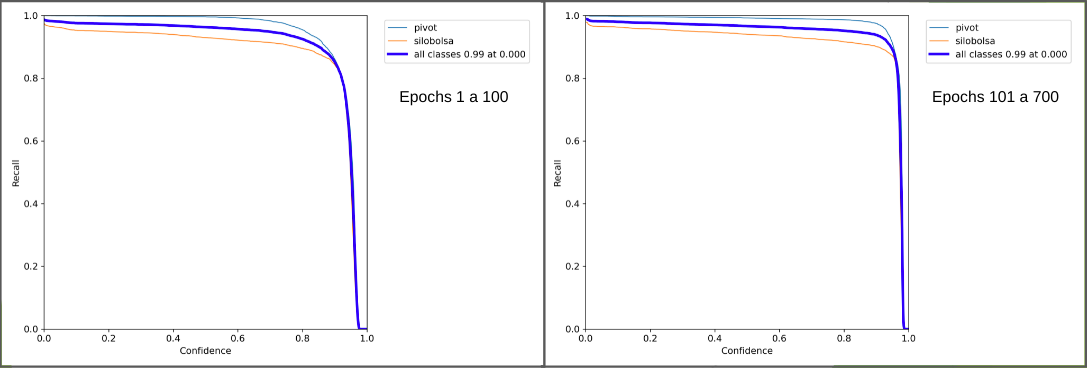
\includegraphics[width=1\textwidth]{img/Recall.png}
    \caption{Recall}
    \label{fig:recall}
\end{figure}

\subsubsection{Precisión/Recall}

De acuerdo a lo mencionado anteriormente, podemos resumir que:\\

\textbf{Precisión:} ¿Cuántas veces, lo que mi modelo dice, es realmente cierto?

\textbf{Recall:} ¿Cuántas veces mi modelo es capaz de identificar la verdad?\\

Al relacionar ambas métricas, podemos decir que, la Precisión se centra en lo que modelo dice y luego lo compara con la realidad. Por otro lado, Recall parte de la realidad, y después evalúa que tan bueno es el modelo para reconocerla.\\
 
\textbf{Resultado obtenido}\\

En la Figura \ref{fig:precision/recall} podemos observar la curva de Precisión/Recall obtenida para la detección de Silobolsas y Pivot desde la Epoch 1 al 100 y de la Epoch 101 a la 700.\\

\begin{figure}[h!]
    \centering
    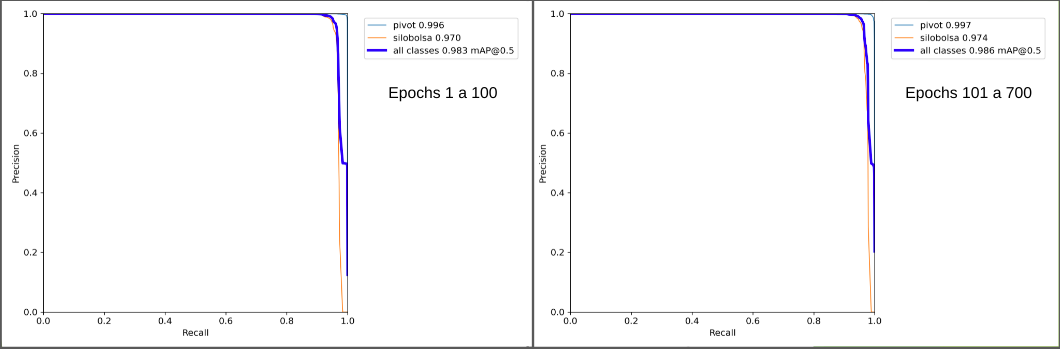
\includegraphics[width=1\textwidth]{img/Precision-Recall.png}
    \caption{Precisión/Recall}
    \label{fig:precision/recall}
\end{figure}

\newpage
\subsubsection{F1 Score}
Es el promedio ponderado de la Precisión y el Recall. Por lo tanto, esta métrica, tiene en cuenta tanto falsos positivos como falsos negativos. Su fórmula es:   \[F1 Score=2*\frac{Recall * Precision}{Recall + Precision}\] \\


\textbf{Resultado obtenido}\\

En la Figura \ref{fig:f1-score} podemos observar la curva de F1 Score obtenida para la detección de Silobolsas y Pivot desde la Epoch 1 al 100 y de la Epoch 101 a la 700.
\begin{figure}[h!]
    \centering
    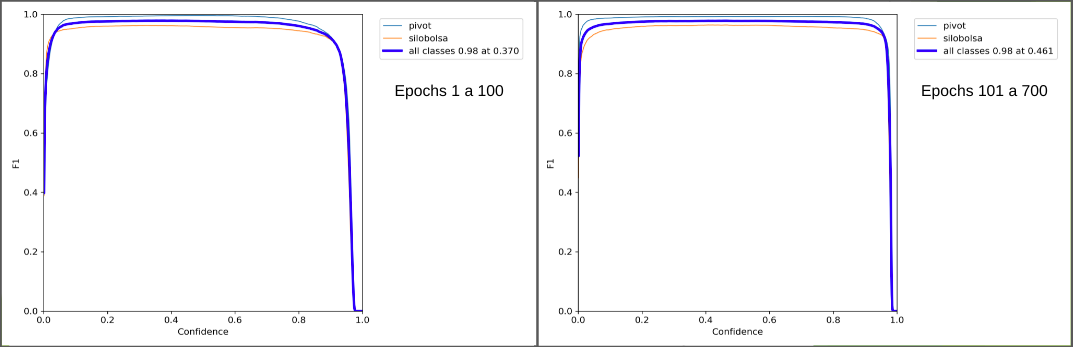
\includegraphics[width=1\textwidth]{img/F1-Score.png}
    \caption{Curva F1 Score}
    \label{fig:f1-score}
\end{figure}


\subsubsection{Loss Function o Función de Pérdida y Precisión Media Promedio (mAP, Mean Average Precision)}
En las siguientes imágenes se exponen los valores que toman las tres loss functions del modelo (bounding box, detección de objeto, clasificación) para los conjunto de validación y testeo; así como también las curvas de precisión, recall y mAP generales (ver figuras \ref{fig:loss-functions-map-100} y \ref{fig:loss-functions-map-700}).\\


\begin{figure}
    \centering
    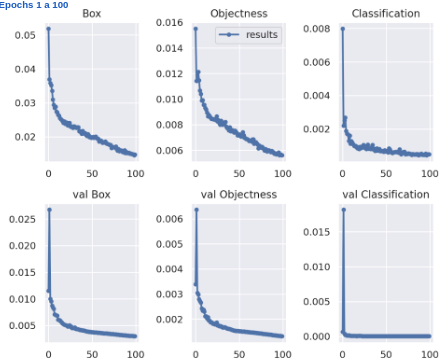
\includegraphics[width=0.8\textwidth]{img/resultados_finales_100_part1.png}
    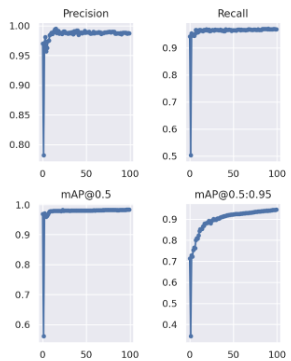
\includegraphics[width=0.5\textwidth]{img/resultados_finales_100_part2.png}
    \caption{Loss Function y mAP. Primeras 100 epochs.}
    \label{fig:loss-functions-map-100}
\end{figure}\\

Antes de comenzar a con los resultados, vamos a definir lo que es un \textbf{epoch}, término que vamos a utilizarlo para explicar los resultados obtenidos.\\

\textbf{Epoch:} Dentro del contexto del aprendizaje automático, epoch se puede describir como un ciclo completo a través de todo el conjunto de datos de entrenamiento e indica la cantidad de pasadas que el algoritmo ha completado durante ese entrenamiento. Es decir, un epoch se compone en última instancia de lotes de datos e iteraciones, cuya suma en última instancia equivaldrá a una época.
\\
Luego de las primeras 100 epochs (o épocas) de entrenamiento, se observan los siguientes resultados:
\begin{itemize}
    \item En cuanto a métricas, los resultados ya eran muy buenos al finalizar la epoch 100.
    \item Las tres loss functions de validación continuaban bajando al finalizar el entrenamiento, lo cual indicaba que aún había lugar para continuar mejorando los resultados, sin overfitting o sobreajuste.
    \item La loss de validación de clasificación, sin embargo, parecía haber llegado a un mínimo.
\end{itemize}

\begin{figure}
    \centering
    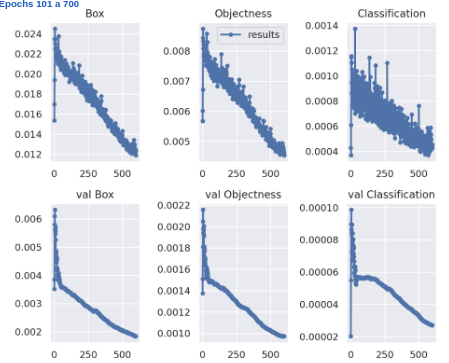
\includegraphics[width=0.9\textwidth]{img/resultados_finales_700_part1.png}
    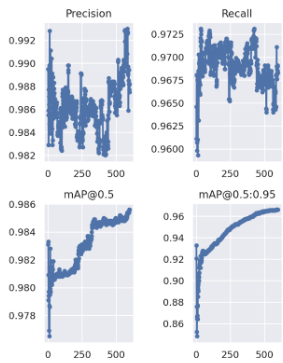
\includegraphics[width=0.6\textwidth]{img/resultados_finales_700_part2.png}
    \caption{Loss Function y mAP. Epochs 101 a 700.}
    \label{fig:loss-functions-map-700}
\end{figure}
Al finalizar las siguientes 600 epochs, se observan los siguientes resultados:
\begin{itemize}
    \item La precisión y recall oscilaron entre valores altos, superiores al 96\%.
    \item El mAP continuó aumentando. En particular fue muy positiva la mejora en el mAP con barrido de IoU (0.5 a 0.95).
    \item Las loss functions de clasificación y validación continuaron bajando, pero sus valores ya eran extremadamente bajos. Quizás quedó algo de lugar para continuar con el entrenamiento, pero se optó por continuar con los siguientes objetivos del proyecto, ya que los resultados cumplían con las expectativas.
\end{itemize}

\newpage
\subsubsection{Matriz de Confusión}
La siguiente matriz de confusión muestra el porcentaje de objetos que el modelo predijo correctamente contra los incorrectos y contra las omisiones.

\begin{figure}
    \centering
    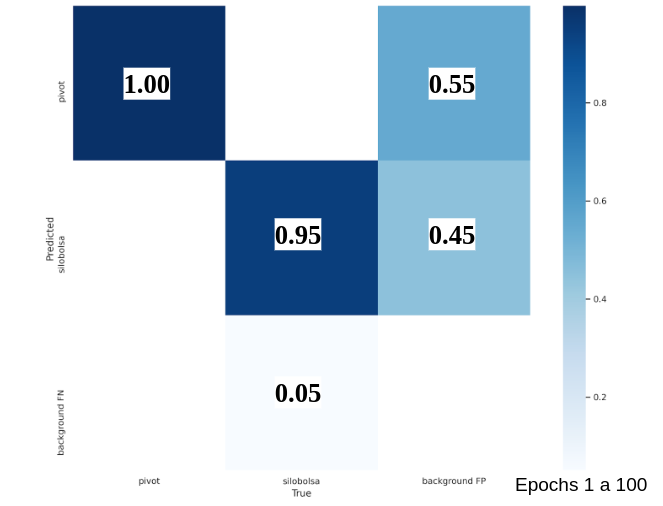
\includegraphics[width=1\textwidth]{img/matriz_confusion_100.png}
    \caption{Matriz de Confusión. Primeras 100 epochs.}
    \label{fig:matriz-confusion-100}
\end{figure}
Al finalizar las primeras 100 epochs, se ve en el gráfico de la izquierda que las detecciones de pivotes son excelentes, es decir, cada pivote fue reconocido, por eso el resultado 1.00. Sin embargo, de las falsas predicciones (FP), más de la mitad de las mismas eran de pivote (55\%). Por otro lado, en el caso de las silobolsas, se detectaron correctamente el 95\% de las mismas, con una proporción de FP de 45\%.

\newpage
Al finalizar la segunda etapa de entrenamiento de 600 epochs, vemos que el porcentaje de silobolsas detectado subió un 1\%, mientras que la mayor diferencia se ve en la distribución de FP, con solo 33\% de pivotes mal detectados y un 67\% de silobolsas. En este caso se aprecia claramente un aumento de la precisión a costa de una disminución de la recall.

\begin{figure}[t!]
    \centering
    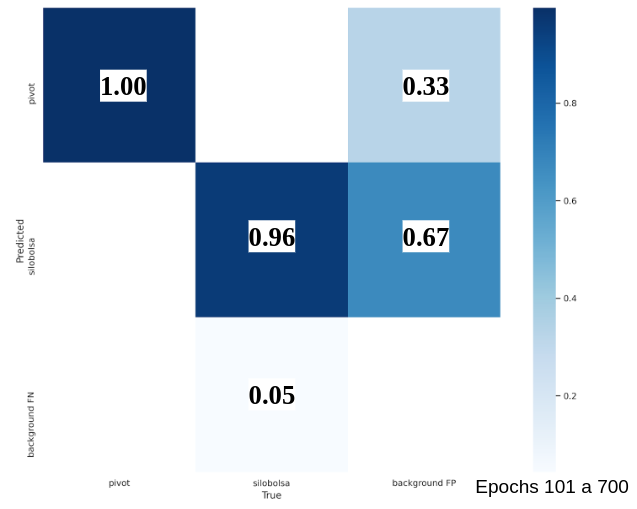
\includegraphics[width=1\textwidth]{img/matriz_confusion_700.png}
    \caption{Matriz de Confusión. Epochs 101 a 700.}
    \label{fig:matriz-confusion-700}
\end{figure}\\

\newpage
\subsection{Despliegue}
\begin{figure}
    \centering
    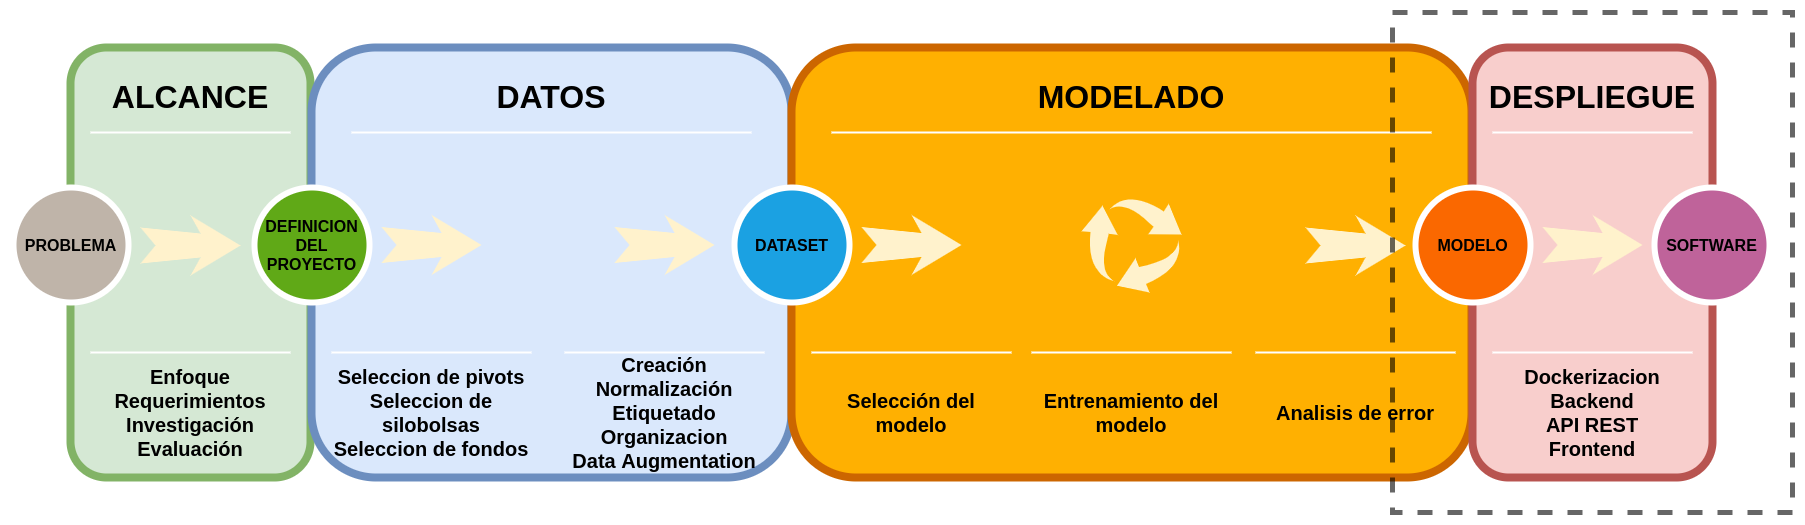
\includegraphics[width=1.2\textwidth,center]{img/Wokflow - despliegue.drawio.png}
    \caption{Workflow: Etapa de Despliegue}
    \label{fig:workflow - despliegue}
\end{figure}
Para la etapa de despliegue se optó por hacer uso de los dos contenedores Docker descriptos lineas arriba: uno corriendo el Backend y otro el Frontend. Este enfoque permite que el software en su totalidad sea fácilmente portado a diferentes sistemas.

\begin{figure}
    \centering
    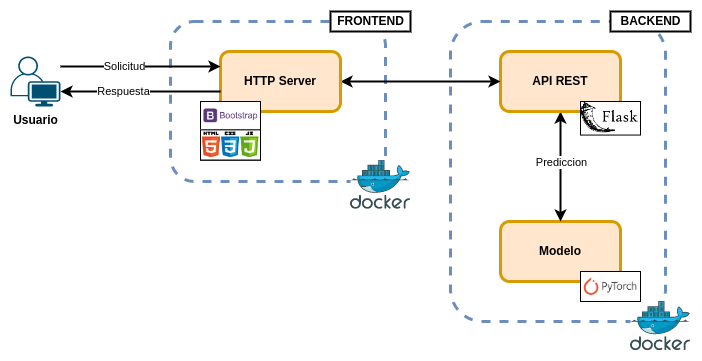
\includegraphics[width=1\textwidth,center]{img/BE - API - FE.drawio.png}
    \caption{Arquitectura del Software Implementado}
    \label{fig:be - api - fe}
\end{figure}
\newpage